\documentclass[10pt]{article}

\usepackage[utf8]{inputenc}
\usepackage[T1]{fontenc}
\usepackage{lmodern}
\usepackage[margin=0.9in]{geometry}
\usepackage{graphicx}
\usepackage{booktabs}
\usepackage{amsmath}
\usepackage{amssymb}
\usepackage{algorithm}
\usepackage{algpseudocode}
\usepackage{hyperref}
\usepackage{multirow}
\usepackage{array}
\usepackage{xcolor}
\usepackage{float}
\usepackage{subcaption}
\captionsetup[subfigure]{justification=centering}
\usepackage{listings}
\usepackage{microtype}

\lstset{
  language=Python,
  basicstyle=\ttfamily\small,
  keywordstyle=\color{blue},
  stringstyle=\color{red},
  commentstyle=\color{gray},
  showstringspaces=false,
  frame=single,
  breaklines=true,
  aboveskip=6pt,
  belowskip=6pt,
}

\graphicspath{{./}}

\title{Cache-DiT: A Unified PyTorch-Native Inference Engine \\ for Diffusion Transformers}
\date{}

\begin{document}

% ---- Custom title page ----
\begin{center}
{\LARGE\bfseries Cache-DiT: A Unified PyTorch-Native Inference Engine \\[4pt] for Diffusion Transformers\par}
\vspace{10pt}
{\large
\mbox{Yanjun~Qiu}\textsuperscript{*},~~\mbox{Zhangqiu~Yu}\textsuperscript{*},~~\mbox{Hua~Xiao}\textsuperscript{\dag},~~\mbox{Xiuquan~Hao}\textsuperscript{\dag} \\
\mbox{Dengfeng~Zhang}\textsuperscript{\dag},~~\mbox{Yunqing~Li}\textsuperscript{\dag},~~\mbox{Guiping~Du}\textsuperscript{\dag},~~\mbox{Wangpeng~Zhan}\textsuperscript{\dag} \\
\mbox{Xiaoyu~Zhang}\textsuperscript{\ddag},~~\mbox{Song~Lin}\textsuperscript{\ddag} \\[6pt]
vipshop.com
\par}
\end{center}
\footnotetext[1]{\textsuperscript{*}Equal contribution (co-first authors).}
\footnotetext[2]{\textsuperscript{\dag}Equal contribution (co-second authors).}
\footnotetext[3]{\textsuperscript{\ddag}GitHub contributors.}
\vspace{4pt}
% ---- End custom title ----

% ============================================================================
% 1. Abstract
% ============================================================================
\begin{abstract}
Diffusion Transformers (DiTs) have become the dominant architecture for high-quality image and video generation, but their inference remains computationally expensive due to three compounding bottlenecks: (1) temporal redundancy across sequential denoising steps, (2) quadratic attention complexity on long sequences, and (3) massive model sizes that exceed GPU memory. Existing approaches address these challenges in isolation---cache methods reduce step-wise computation, parallelism distributes sequence and parameter loads, quantization compresses weights, and CPU offloading extends memory capacity---but no framework unifies them into a single, composable system.

We present Cache-DiT, a PyTorch-native inference engine that unifies \textbf{hybrid cache acceleration, comprehensive parallelism, W4A4 quantization, and bucket-style layerwise CPU offload} in a single framework. Cache-DiT introduces (1) \textbf{Dual Block Cache (DBCache)} together with \textbf{Steps Computation Mask (SCM)} and \textbf{TaylorSeer}, achieving \textbf{up to $3.9\times$ speedup with negligible quality loss} and \textbf{up to $5.7\times$ in aggressive mode} on DrawBench; (2) a \textbf{comprehensive hybrid parallelism stack}, including \textbf{Ulysses Anything Attention (UAA)} for arbitrary sequence lengths and head counts; (3) a \textbf{calibration-free dynamic quantization (DQ) mode} for SVDQuant W4A4 that removes the need for representative calibration data; and (4) a \textbf{bucket-style layerwise offload strategy} that achieves \textbf{about $5\%$ latency overhead} compared to no-offload execution under constrained GPU memory budgets. All features are exposed through a single \texttt{enable\_cache()} API and can be freely composed, enabling \textbf{up to $5.52\times$ end-to-end speedup} on a single NVIDIA L20 GPU for FLUX.1-dev.

Cache-DiT supports \textbf{70+ DiT models} and is already integrated into \textbf{vLLM-Omni, SGLang Diffusion, TensorRT-LLM, ComfyUI}, and other production frameworks. The engine is open-source and available at \url{https://github.com/vipshop/cache-dit}.
\end{abstract}

% ============================================================================
% 2. Introduction
% ============================================================================
\section{Introduction}

Diffusion Transformers (DiTs)~\cite{peebles2023scalable} have emerged as the leading architecture for high-fidelity generative modeling, powering state-of-the-art image generation (FLUX~\cite{flux2024}, SD3~\cite{esser2024scaling}, Qwen-Image~\cite{qwenimage2025}), video generation (Wan~\cite{wan2025}, HunyuanVideo~\cite{hunyuanvideo2024}, CogVideoX~\cite{yang2024cogvideox}), and image editing (Z-Image~\cite{zimage2025}, Ovis-Image~\cite{ovisimage2025}). The core of a DiT model is a transformer backbone that iteratively denoises latent representations across 20--50 steps, with each step performing a full forward pass through dozens of transformer blocks. While DiTs deliver remarkable generation quality, their inference cost is prohibitive for real-world deployment: a single 1024$\times$1024 image generated by FLUX.1-dev takes over 24 seconds on an NVIDIA L20 GPU.

Three fundamental bottlenecks compound this cost. \textbf{First}, consecutive denoising steps exhibit significant temporal redundancy---neighboring steps produce highly similar intermediate features---yet standard inference recomputes every transformer block at every step. \textbf{Second}, the attention mechanism scales quadratically with sequence length $O(N^2)$, and high-resolution generation (e.g., 2048$\times$2048 for FLUX.2-dev) produces sequences of tens of thousands of tokens. \textbf{Third}, modern DiT models are massive, with large-scale models requiring over 100\,GiB of GPU memory in full precision, exceeding the capacity of most datacenter GPUs.

The research community has developed effective techniques for each bottleneck in isolation. Cache-based methods~\cite{ma2023deepcache, liu2025teacache, silveria2025chipmunk, chen2024deltadit} exploit temporal redundancy by skipping computation on redundant steps or blocks. Parallelism techniques~\cite{jacobs2023ulysses, liu2023ring, fang2024xdit} distribute the sequence or parameter load across multiple GPUs through context parallelism (CP) and tensor parallelism (TP). Quantization methods~\cite{li2025svdquant, hanlab2025nvfp4} compress weights and activations to 4-bit precision. CPU offloading~\cite{diffusers2024} moves model weights to CPU memory between layers. However, these techniques operate in \textit{separate codebases} with \textit{incompatible APIs}---a practitioner who wants to combine cache acceleration with parallelism and quantization must manually integrate three different libraries, each with its own configuration schema, model patching logic, and version constraints. Worse, some combinations are fundamentally incompatible across library boundaries (e.g., a parallelism library's sequence sharding may conflict with a cache library's block-level state management).

We argue that these optimizations are not merely compatible---they are \textit{orthogonal and synergistic}. Cache exploits step-wise redundancy, parallelism distributes per-step loads, and quantization compresses per-layer parameters. None of them modifies the fundamental computation in a way that precludes the others. What is missing is a \textit{unified system design} that treats them as composable layers atop a model-agnostic abstraction.

\textbf{Cache-DiT} is a PyTorch-native inference engine that unifies hybrid cache acceleration, comprehensive parallelism, W4A4 quantization, and bucket-style layerwise CPU offload into a single framework, accessible through one line of code: \texttt{cache\_dit.enable\_cache(pipe)}. The key architectural insight is a \textbf{BlockAdapter} registry---a model-agnostic mechanism that discovers and instruments DiT transformer blocks across any HuggingFace Diffusers pipeline. Once instrumented, the four optimization layers (cache, parallelism, quantization, offload) attach as composable middleware, each operating within its own orthogonal dimension. This design enables any combination of optimizations to be stacked without conflict.

Our contributions are:

\begin{enumerate}
    \item \textbf{A unified DiT inference framework} that makes hybrid cache, distributed parallelism, W4A4 quantization, and layerwise CPU offload freely composable---all through a single \texttt{enable\_cache()} API, working across 70+ DiT models without per-model code changes.
    \item \textbf{A comprehensive hybrid parallelism system} spanning Context Parallelism (Ulysses, Ring, USP), Tensor Parallelism, and Extra Parallelism (VAE-P, TE-P, CN-P), which together enable \textbf{5D parallelism} (CP + TP + VAE-P + TE-P + CN-P) on large DiT models. The system further includes \textbf{Ulysses Anything Attention} (UAA) for arbitrary sequence lengths and head counts, \textbf{Async Ulysses} for overlapping QKV projection with communication, and \textbf{FP8 communication} for bandwidth reduction---all configurable within a single \texttt{ParallelismConfig} object.
    \item \textbf{Dual Block Cache (DBCache)}, a training-free cache algorithm that uses a dual-block mechanism ($F_n$ front blocks for stable L1-diff estimation, $B_n$ back blocks for auto-scaling) together with a Steps Computation Mask (SCM) and TaylorSeer calibrator. DBCache achieves up to $3.9\times$ speedup with negligible image quality loss on DrawBench, and up to $5.7\times$ in aggressive mode.
    \item \textbf{A calibration-free dynamic quantization (DQ) mode} for SVDQuant W4A4 that eliminates the need for representative calibration data. We identify that SVDQuant's runtime dynamically recomputes activation scales from current inputs---making the offline calibration step non-essential for many use cases.
    \item \textbf{Bucket-style layerwise CPU offload} that achieves about $5\%$ latency overhead over no-offload execution under constrained GPU memory, using asynchronous bucket-level prefetch with configurable persistent bins.
    \item \textbf{Production-grade community adoption}: Cache-DiT is documented or integrated in vLLM-Omni, SGLang Diffusion, Diffusers optimization guides, TensorRT-LLM upstream work, ComfyUI, SD.Next, and other downstream frameworks.
\end{enumerate}

Experiments across 6 model families (FLUX.1/2, Qwen-Image, Z-Image, LTX-2, and Longcat-Image-Edit) on NVIDIA L20, H100, and H800 GPUs demonstrate Cache-DiT's effectiveness: DBCache alone provides $1.6$--$2.9\times$ speedup with controllable quality trade-offs; Ulysses-2 parallelism scales FLUX.1-dev inference from $9.30$\,s to $6.04$\,s on H100; combining cache, Ulysses-2, compilation, and FP8 quantization yields $4.84\times$ end-to-end speedup (from $9.30$\,s to $1.92$\,s) on H100, and $5.52\times$ on L20. On the large FLUX.2-dev model, hybrid Ulysses-4 + TP-2 parallelism reduces latency from $21.37$\,s (TP-8) to $15.21$\,s, and further to $7.73$\,s with cache enabled.

% ============================================================================
% 3. Background & Related Work
% ============================================================================
\section{Background and Related Work}

\subsection{DiT Inference Pipeline}

A DiT inference pipeline consists of four components: a text encoder that embeds the input prompt, a variational autoencoder (VAE) that compresses images into a latent space, a diffusion scheduler that governs the iterative denoising process, and the DiT transformer backbone that performs the actual denoising. At each denoising step $t$, the transformer takes a noisy latent $z_t$ and conditioning embeddings as input, and predicts the noise $\epsilon_\theta(z_t, t, c)$. The process repeats for $T$ steps (typically 20--50), with the final latent decoded by the VAE into the output image or video frame.

The transformer backbone dominates inference cost, accounting for $>95\%$ of total latency and memory. It consists of stacked transformer blocks, each containing self-attention, cross-attention, and feed-forward network (FFN) sub-layers. The self-attention complexity $O(N^2 d)$ grows quickly with spatial resolution---FLUX.2-dev at $2048\times2048$ produces sequences of $N\approx 16\text{K}$ tokens per image. Modern DiT models range from a few billion parameters to large-scale models requiring over 100\,GiB of GPU memory in BF16 precision.

\subsection{Cache Acceleration for DiTs}

The observation that consecutive denoising steps produce similar features has motivated a rich line of cache-based acceleration methods. DeepCache~\cite{ma2023deepcache} caches high-level features from earlier steps and reuses them in later steps, achieving $\sim$2$\times$ speedup for UNet-based diffusion models. TeaCache~\cite{liu2025teacache} and TaylorSeer~\cite{liu2025taylorseer} extend this idea to DiTs with learned or Taylor-expansion-based step prediction. $\Delta$-DiT~\cite{chen2024deltadit}, FORA~\cite{selvaraju2024fora}, ToCa~\cite{zou2025toca}, DuCa~\cite{zou2024duca}, and FoCa~\cite{zheng2025foca} propose progressively more sophisticated cache decision criteria based on feature differences, attention maps, or learned predictors. Chipmunk~\cite{silveria2025chipmunk} combines caching with structured pruning. These methods demonstrate that DiT inference contains substantial temporal redundancy, but each is implemented as a standalone patch to specific model architectures, making it difficult to combine with other optimizations or apply to new models.

\subsection{Parallelism for Diffusion Models}

Distributing DiT inference across multiple GPUs has been explored through several paradigms. Sequence parallelism methods split the input sequence across devices: Ulysses~\cite{jacobs2023ulysses} performs all-to-all communication on attention heads, while Ring Attention~\cite{liu2023ring} rotates key-value blocks through peer-to-peer transfers. USP (Unified Sequence Parallelism) combines both into a hybrid scheme. Tensor parallelism~\cite{narayanan2021megatron} shards individual weight matrices across devices. xDiT~\cite{fang2024xdit} provides a practical framework for CP/TP-style distributed DiT execution. DistriFusion~\cite{li2024distrifusion} and PipeFusion~\cite{wang2024pipefusion} study distributed diffusion execution under different partitioning schemes, with PipeFusion specifically emphasizing patch-level pipelining. Despite this progress, several practical challenges remain: many CP implementations still require the sequence length and/or the head count to be divisible by the parallelism degree, hybrid combinations of CP and TP are often exposed through fragmented configuration surfaces, and communication efficiency remains sensitive to synchronization overhead, all-to-all scheduling, and datatype choices. These constraints motivate support for mechanisms such as UAA, Async Ulysses, and FP8 communication, which make distributed DiT inference easier to apply across more diverse real-world model configurations.

\subsection{Quantization and Offloading}

Post-training quantization (PTQ) compresses model weights and activations to lower bit-widths. For DiTs, SVDQuant~\cite{li2025svdquant} proposes W4A4 quantization by absorbing activation outliers into a low-rank branch computed via SVD, with the residual quantized to INT4. Nunchaku packages highly optimized kernels for this workflow, but its integration path is still largely organized around model-specific adapters and kernel plumbing rather than a single model-agnostic DiT acceleration framework. Recent engineering work also extends SVDQuant-style W4A4 execution to NVFP4-oriented deployment paths on Blackwell GPUs~\cite{hanlab2025nvfp4}. torchao~\cite{torchao2024} provides generic quantization primitives for FP8 and INT4. CPU offloading~\cite{diffusers2024} moves model weights between CPU and GPU to reduce peak memory, but existing sequential and model-level offload schemes often incur substantial transfer overheads that can dominate latency and become impractical for production inference.

\subsection{Positioning of Cache-DiT}

Each line of work above addresses one bottleneck effectively in isolation. Cache-DiT's contribution is to resolve the systems gap left between them: it turns cache acceleration, hybrid parallelism, quantization, and offloading into a single unified framework with one configuration surface and several new system techniques that make these optimizations actually composable in practice. This unification is made possible by the BlockAdapter abstraction (Section~\ref{sec:architecture}), which decouples model-specific instrumentation from optimization logic, and by careful co-design of the composability interfaces (Section~\ref{sec:api}). The result is a system where practitioners can freely stack optimizations (e.g., DBCache + Ulysses-4 + SVDQuant DQ + bucket offload) through a single API call, without writing model-specific glue code or re-implementing each optimization for every new DiT pipeline.

% ============================================================================
% 4. System Design
% ============================================================================
\section{System Design}

\subsection{Architecture Overview}
\label{sec:architecture}

Cache-DiT is built as a composable middleware layer atop HuggingFace Diffusers. Figure~\ref{fig:arch} illustrates the overall architecture. The system consists of four components: (1) a \textbf{BlockAdapter} registry for model-agnostic transformer block discovery, (2) a set of \textbf{composable optimization layers} (cache, parallelism, quantization, offload), (3) a \textbf{unified configuration API}, and (4) a \textbf{backend dispatch} layer for attention and kernel selection.

\begin{figure}[htbp]
\centering

\includegraphics[width=0.92\linewidth]{arch_v2.png}
\caption{Cache-DiT system architecture. The BlockAdapter registry instruments any DiT pipeline, then composable optimization layers (Cache, Parallelism, Quantization, Offload) attach as middleware, all accessible through a single \texttt{enable\_cache()} API.}
\label{fig:arch}
\end{figure}

\textbf{BlockAdapter Registry.} The central design challenge in building a unified DiT inference engine is model diversity. Different DiT architectures (FLUX, SD3, Qwen-Image, Wan, CogVideoX, etc.) have different transformer block structures, forward signatures, and conditioning mechanisms. Cache-DiT addresses this with a \textbf{BlockAdapter}---a per-model descriptor that specifies: (1) how to locate the transformer blocks within the pipeline module tree, (2) the forward signature pattern (e.g., whether the block returns \texttt{(hidden\_states, encoder\_hidden\_states)} or just \texttt{hidden\_states}), and (3) an optional \texttt{PatchFunctor} for model-specific forward method rewriting.

Figure~\ref{fig:forward_pattern} shows the six canonical \textbf{Forward Patterns} that cover the forward signatures of all supported DiT models. Each pattern specifies the input/output tensor order---for example, Pattern~1 expects a single tensor (hidden states in, hidden states out), while Pattern~3 handles dual tensors (hidden states and encoder hidden states in both directions). These patterns allow the cache engine to generically intercept and cache activations regardless of the underlying model architecture. For hybrid models like FLUX.1 that contain multiple block types (e.g., \texttt{transformer\_blocks} and \texttt{single\_transformer\_blocks}) with different forward signatures, the BlockAdapter supports per-block-type pattern assignment through a list of \texttt{ForwardPattern} values.

\begin{figure}[htbp]
\centering
\includegraphics[width=0.88\linewidth]{patterns-v1.png}
\caption{Forward Pattern matching. Cache-DiT defines six canonical forward signature patterns that cover all supported DiT architectures. The BlockAdapter maps each model's transformer blocks to one of these patterns, enabling generic cache injection without per-model code.}
\label{fig:forward_pattern}
\end{figure}

The \texttt{PatchFunctor} mechanism handles models that require forward method rewriting to conform to a standard pattern. For instance, FLUX's \texttt{FluxSingleTransformerBlock} natively returns only \texttt{hidden\_states}, but the cache engine expects the encoder hidden states as well; \texttt{FluxPatchFunctor} rewrites the block's forward method to return \texttt{(encoder\_hidden\_states, hidden\_states)}. The \texttt{BlockAdapterRegister} maps pipeline class name prefixes to their corresponding adapters via lazy import, enabling support for new models by adding a single adapter file without modifying core engine code. Currently, 70+ DiT pipelines are registered.

\textbf{Composable Optimization Layers.} Once the BlockAdapter instruments a pipeline, four optimization layers can be attached in sequence. Each layer operates on an orthogonal dimension of the inference cost and is implemented as a set of hooks or module replacements that do not interfere with one another:

\begin{itemize}
    \item \textbf{Cache layer} wraps each transformer block's forward method to intercept activations, compute residual differences, and skip redundant computations.
    \item \textbf{Parallelism layer} applies distributed sharding and communication plans to attention, transformer linear layers, and optional extra modules (e.g., text encoders, VAE, ControlNet), automatically constructing device meshes and inserting the required collectives.
    \item \textbf{Quantization layer} replaces \texttt{nn.Linear} modules with quantized variants (SVDQuant W4A4 or torchao FP8/INT4), handling weight packing and dynamic activation scaling.
    \item \textbf{Offload layer} attaches pre/post forward hooks to move module weights between CPU and GPU, using bucket-level scheduling for asynchronous overlap.
\end{itemize}

\textbf{Unified API.} All configuration is centralized in a single \texttt{enable\_cache()} call that accepts optional \texttt{DBCacheConfig}, \texttt{ParallelismConfig}, and \texttt{QuantizeConfig} objects. The API validates configuration compatibility (e.g., attention backend support for context parallelism) and applies optimizations in a fixed order: instrumentation $\rightarrow$ parallelism $\rightarrow$ cache $\rightarrow$ quantization. Layerwise offload is applied separately via \texttt{layerwise\_offload()} for memory-constrained scenarios.

\subsection{Unified Hybrid Cache Engine}

Cache-DiT's cache engine combines four complementary strategies into a single configurable pipeline: DBCache (dual-block residual caching), SCM (steps computation mask), TaylorSeer (Taylor-expansion-based step prediction), and DBPrune (dynamic block pruning). Figure~\ref{fig:dbcache_arch} illustrates the overall cache engine architecture.

\begin{figure}[htbp]
\centering
\includegraphics[width=0.88\linewidth]{dbcache-v1.png}
\caption{DBCache architecture. The cache engine intercepts each transformer block's forward pass, computes L1 residual differences against cached states from the previous step, and decides whether to skip or compute each block based on the dual-block ($F_n$, $B_n$) policy and residual threshold $\tau$.}
\label{fig:dbcache_arch}
\end{figure}

\subsubsection{DBCache: Dual Block Cache}

The core idea of DBCache is to exploit the temporal redundancy of intermediate features across denoising steps without training. For each transformer block at step $t$, DBCache compares the current block output $h_t^{(l)}$ against the cached output from the previous step $h_{t-1}^{(l)}$. If the L1 difference falls below a threshold $\tau$, the block is skipped and the cached output is reused.

A naive per-block cache suffers from error accumulation: early blocks may produce acceptable differences, but the errors compound through subsequent blocks, degrading final image quality. DBCache addresses this with a \textbf{dual-block mechanism} parameterized by two integers $(F_n, B_n)$:

\begin{itemize}
    \item \textbf{$F_n$ front compute blocks}: The first $F_n$ transformer blocks are \textit{always} computed. These blocks fit the information at the current timestep $t$ and produce a stable L1-diff signal for downstream cache decisions. Since earlier blocks capture coarser features that change more across steps, forcing their computation provides a reliable reference.
    \item \textbf{$B_n$ back calibration blocks}: The last $B_n$ blocks are also always computed. These blocks act as an \textit{auto-scaler} that refines the approximate hidden states produced by cached intermediate blocks, absorbing accumulated errors before the output reaches the next timestep.
\end{itemize}

Blocks between positions $F_n$ and $L-B_n$ use the residual cache: if $\|h_t^{(l)} - h_{t-1}^{(l)}\|_1 < \tau$, skip computation and reuse $h_{t-1}^{(l)}$; otherwise, compute normally and update the cache. The threshold $\tau$ controls the speed-quality trade-off, with typical values ranging from 0.08 (conservative) to 0.20 (aggressive). Figure~\ref{fig:dbcache} illustrates this dual-block mechanism.

\begin{figure}[htbp]
\centering
\includegraphics[width=0.85\linewidth]{dbcache-fnbn-v1.png}
\caption{DBCache dual-block mechanism. The first $F_n$ blocks are always computed to provide a stable L1-diff reference; the last $B_n$ blocks serve as auto-scalers that refine cached intermediate outputs. Middle blocks skip computation when the residual L1 difference falls below threshold $\tau$.}
\label{fig:dbcache}
\end{figure}

DBCache also includes a warmup phase (controlled by \texttt{max\_warmup\_steps}) during which no caching occurs, allowing the model to establish stable features before cache decisions begin. The \texttt{max\_continuous\_cached\_steps} parameter limits consecutive cache hits to prevent drift.

\subsubsection{SCM: Steps Computation Mask}

Inspired by LeMiCa~\cite{gao2025lemica} and EasyCache~\cite{zhou2025easycache}, the Steps Computation Mask (SCM) applies a non-uniform cache schedule across denoising steps. The key observation is that early denoising steps are more sensitive to cache errors---caching early amplifies downstream degradation, while caching later steps has minimal impact. SCM defines a binary mask $M \in \{0,1\}^T$ where $M_t=1$ means ``compute all blocks at step $t$'' and $M_t=0$ means ``apply DBCache at step $t$.''

Cache-DiT provides pre-configured SCM strategies that users can adapt to arbitrary step counts. For example, on a 28-step schedule, four presets are available: \texttt{slow} (18 compute steps, 10 cache steps), \texttt{medium} (15 compute steps, 13 cache steps), \texttt{fast} (11 compute steps, 17 cache steps), and \texttt{ultra} (8 compute steps, 20 cache steps).
Users can also define custom masks for arbitrary step counts. SCM can be combined with \texttt{dynamic} mode, where the mask is adjusted at runtime based on the observed residual diff trajectory.

\subsubsection{TaylorSeer Calibrator}

TaylorSeer~\cite{liu2025taylorseer} predicts the hidden states at step $t+1$ using a Taylor expansion around the current step's states. When combined with DBCache, TaylorSeer serves as a \textit{pre-cache} predictor: if the predicted next-step features are sufficiently close to the cached features, the cache can be engaged earlier. In practice, TaylorSeer is most effective when paired with DBCache configurations that use $B_n=0$ (no back calibration blocks), since the prediction reduces the need for back-block refinement.

\subsubsection{DBPrune: Dynamic Block Pruning}

DBPrune extends DBCache with per-block pruning decisions: instead of caching the entire block output, it selectively prunes individual sub-layers within a block based on their L1 distance from the previous step. Blocks that are pruned save both computation and memory bandwidth. DBPrune supports configurable pruning ratios (24\%--60\%) and can exclude specific block IDs from pruning (e.g., the first and last blocks).

\begin{figure}[H]
\centering
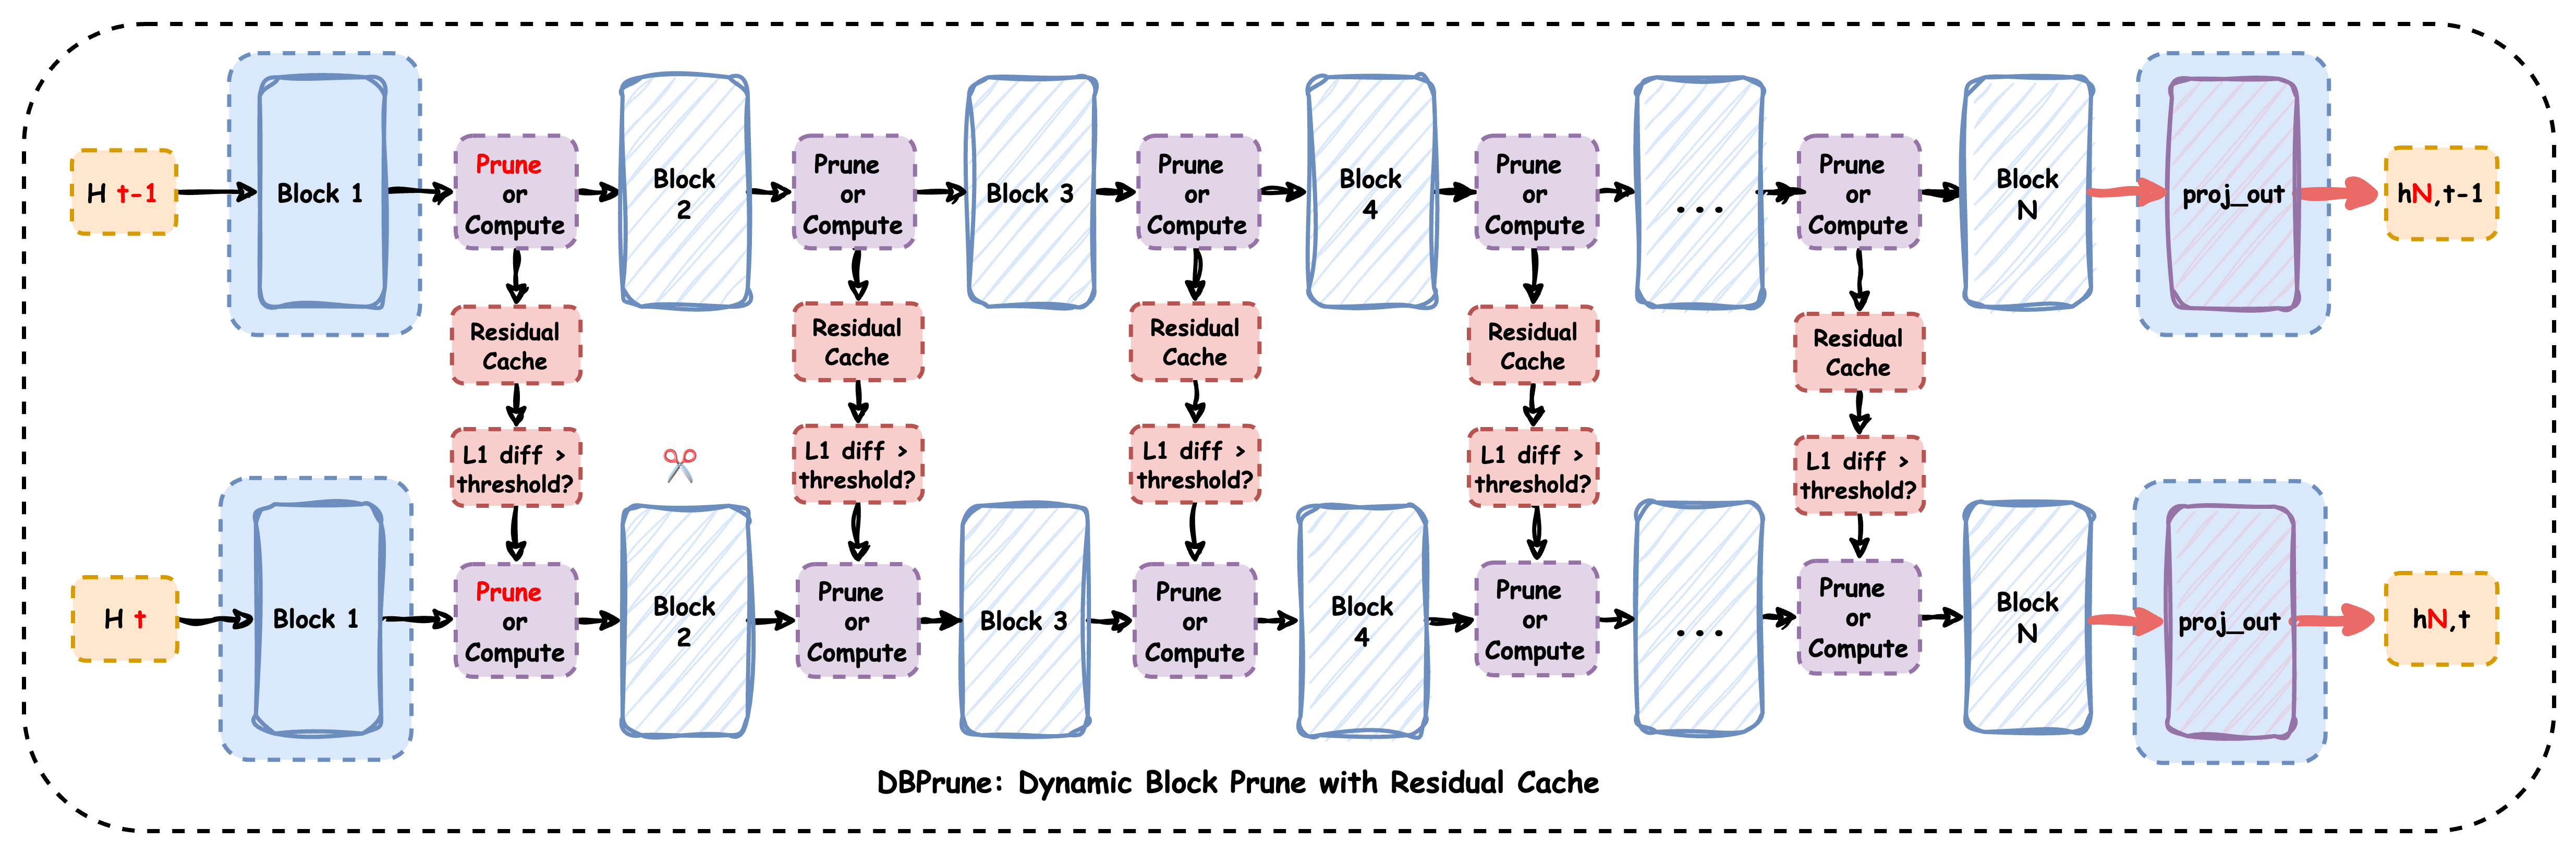
\includegraphics[width=0.92\linewidth]{../../docs/assets/dbprune.png}
\caption{DBPrune algorithm flow. Each block caches hidden states and residuals, computes an L1-distance-based prune decision at the next step, and either executes the block normally or reconstructs the output from cached residuals when the block is pruned.}
\label{fig:dbprune_flow}
\end{figure}

As illustrated in Figure~\ref{fig:dbprune_flow}, DBPrune first caches each block's hidden states and residuals, then evaluates the inter-step L1 distance to decide whether the block should be executed or skipped. If the distance falls below the pruning threshold, the block output is approximated from the cached residual path; otherwise, the full block is recomputed and the cache is refreshed for later steps.

\subsubsection{CFG Cache Support}

For classifier-free guidance (CFG), DiT models perform two forward passes per step: one conditional (with text embedding) and one unconditional. Cache-DiT supports separate cache states for CFG and non-CFG passes via the \texttt{enable\_separate\_cfg} flag, and allows configurable CFG-first or CFG-second computation order. For fused-execution pipelines, the adapter can still expose separate CFG cache states when the model structure permits; otherwise the runtime falls back to a shared cache path consistent with the fused forward.

\subsection{Comprehensive Parallelism}
\label{sec:parallelism}

Cache-DiT provides a complete parallelism toolkit spanning context parallelism, tensor parallelism, and extra-module parallelism, all configurable through a single \texttt{ParallelismConfig} object.

\subsubsection{Context Parallelism: Ulysses, Ring, and USP}

Three context parallelism strategies are supported, selectable by setting \texttt{ulysses\_size} and/or \texttt{ring\_size}:

\textbf{Ulysses Attention} shards the input sequence along the head dimension. Before attention, an all-to-all communication redistributes QKV tensors so that each device holds the full sequence for a subset of heads. After attention, a second all-to-all gathers the output. Ulysses preserves exact attention semantics (no approximation) and requires $\mathcal{O}(Nhd/W)$ memory per device, where $W$ is the parallelism degree. Its main limitation is the requirement that the number of attention heads $h$ be divisible by $W$.

\textbf{Ring Attention} partitions the sequence into $W$ contiguous chunks, with each device holding one chunk. During attention computation, key-value blocks are rotated through peer-to-peer transfers in a ring topology, allowing each device to compute the full attention for its local query chunk. Ring Attention has no head-count constraint but incurs higher communication volume than Ulysses.

\textbf{USP (Unified Sequence Parallelism)} combines Ulysses and Ring into a hybrid 2D strategy: an outer Ulysses all-to-all across $\text{ulysses\_size}$ groups, with inner Ring P2P within each group. This enables scaling to higher parallelism degrees while balancing communication and memory trade-offs.

\subsubsection{UAA: Ulysses Anything Attention}

Standard Ulysses Attention imposes two divisibility constraints in practice: the sequence length of the hidden states must be divisible by the parallelism degree $W$, and the vanilla head-sharding path also expects the number of attention heads $h$ to be divisible by $W$. Many real-world DiT models violate one or both conditions: Z-Image-Turbo uses $h=30$ (not divisible by 4), while Qwen-Image at non-standard resolutions produces sequence lengths not divisible by $W$. Cache-DiT introduces \textbf{Ulysses Anything Attention (UAA)}, which removes both constraints within a unified attention path.

UAA works by padding the head dimension to the next multiple of $W$ during the all-to-all communication phase, and masking out the padded heads during attention computation. For sequence length alignment, UAA gathers the actual sequence lengths across devices and uses them to construct the attention mask, avoiding the need for zero-padding the sequence dimension. The key insight is that UAA resolves the two divisibility constraints through two separate lightweight mechanisms: head-count mismatch is handled by padding/unpadding around all-to-all, while sequence-length mismatch is handled by exchanging true per-rank sequence lengths and masking from the real lengths. Only by addressing both constraints together can Ulysses become broadly usable across arbitrary DiT resolutions and head configurations, while still incurring only minimal extra communication overhead (typically {$<0.1\%$} of total latency) compared to standard Ulysses.

\subsubsection{Async Ulysses and FP8 Communication}

Two orthogonal communication optimizations further reduce Ulysses overhead:

\textbf{Async Ulysses QKV Projection} overlaps the Q, K, V linear projections with the subsequent all-to-all communication. Inspired by VeOmni's async Ulysses design~\cite{ma2025veomni}, Cache-DiT adapts this idea to DiT inference and schedules the projection for head subsets to begin while earlier subsets are already communicating. This is implemented via per-model \texttt{AsyncUlyssesPlanner} instances that rewrite the QKV projection code to insert asynchronous communication primitives, as illustrated in Figure~\ref{fig:async_ulysses}.

\begin{figure}[H]
\centering

\includegraphics[width=0.82\linewidth]{async_ulysses.png}
\caption{Async Ulysses QKV Projection: overlapping projection with all-to-all communication.}
\label{fig:async_ulysses}
\end{figure}

\textbf{FP8 Ulysses} reduces all-to-all communication volume by quantizing the Q, V, and output tensors to FP8 before transmission. The K tensor is kept in BF16/FP16 to preserve softmax precision. Per-token FP8 quantization and dequantization kernels are implemented in Triton and CuTeDSL backends, as illustrated in Figure~\ref{fig:fp8_ulysses}.

\begin{figure}[H]
\centering

\includegraphics[width=0.82\linewidth]{async_ulysses_fp8.png}
\caption{FP8 Ulysses: FP8-quantized all-to-all communication with BF16 K preservation.}
\label{fig:fp8_ulysses}
\end{figure}

\subsubsection{Tensor Parallelism and Hybrid 2D/3D/5D Parallelism}

Tensor parallelism (TP) shards individual weight matrices across devices, reducing per-device memory and compute. Cache-DiT's TP uses PyTorch's \texttt{DTensor} API with per-model planners that specify which modules to shard and how. TP is fully composable with CP: setting both \texttt{ulysses\_size} (or \texttt{ring\_size}) and \texttt{tp\_size} to values $>1$ enables hybrid 2D (CP+TP) or 3D (USP+TP) parallelism. The device mesh is automatically constructed as \texttt{[ring, ulysses, tp]}, and hybrid layouts are realized through PyTorch \texttt{DeviceMesh} submeshes so that CP, TP, and higher-dimensional extensions can reuse the same sharding abstraction without model-specific rewrites.

\subsubsection{Extra Parallelism: TE-P, VAE-P, CN-P}

Beyond the transformer backbone, DiT pipelines contain three additional components that can become memory bottlenecks: the text encoder, the VAE decoder, and optional ControlNet modules. Cache-DiT provides \textbf{TE-P} (Text Encoder Parallelism), \textbf{VAE-P} (VAE Parallelism), and \textbf{CN-P} (ControlNet Parallelism), which apply TP sharding to these components using the same \texttt{extra\_parallel\_modules} API. This enables true \textbf{5D parallelism}: CP + TP + TE-P + VAE-P + CN-P, all specified in a single configuration.

\subsection{SVDQuant W4A4 PTQ/DQ}
\label{sec:svdquant}

SVDQuant~\cite{li2025svdquant} is a W4A4 post-training quantization method that absorbs activation outliers into a low-rank branch, enabling aggressive 4-bit quantization of both weights and activations for DiT models. Cache-DiT independently maintains an adapted set of SVDQuant operators and runtime kernels inside its own quantization stack, and builds two production-grade workflows on top: a full PTQ pipeline with calibration and checkpoint serialization, and a calibration-free DQ mode.

\subsubsection{Background: SVDQuant Algorithm}

SVDQuant operates in three stages.

\textbf{Stage 1 (Smoothing).} A SmoothQuant-style per-channel smoothing factor $s \in \mathbb{R}^{K}$ is computed from calibration activations, balancing the quantization difficulty between weights and activations. The original weight matrix $W \in \mathbb{R}^{N \times K}$ is transformed to a smoothed coordinate system: $W_s = W \cdot \mathrm{diag}(s)$.

\textbf{Stage 2 (Low-rank decomposition):} The smoothed weight $W_s$ is decomposed via SVD into a low-rank approximation $L_{\text{up}} L_{\text{down}}$ (of rank $R$) and a residual $W_{\text{res}} = W_s - L_{\text{up}} L_{\text{down}}$. The residual is quantized to INT4 with group size 64, producing packed integer weights $\hat{W}_{\text{res}}$ and per-group scales $w_{\text{scales}}$. The low-rank branch is kept in BF16.

\textbf{Stage 3 (Runtime):} At inference time, the input activation $x$ is first transformed by the inverse smoothing factor: $x_s = x \cdot \mathrm{diag}(s)^{-1}$. The activation is quantized to INT4 per-group, producing dynamic scales $a_{\text{scales}}$ computed from the current input. The main path computes $\hat{y}_{\text{main}} = \text{W4A4-GEMM}(\hat{x}_s, \hat{W}_{\text{res}}, a_{\text{scales}}, w_{\text{scales}})$, and the low-rank path computes $y_{\text{lora}} = (x_s L_{\text{down}}^\top) L_{\text{up}}^\top$. The final output is $y = \hat{y}_{\text{main}} + y_{\text{lora}} + b$.

\textbf{A critical implementation detail} is that the runtime \textit{dynamically recomputes} $a_{\text{scales}}$ from the current activation $x_s$ at every forward pass. The calibration phase only fixes the static smoothing factor $s$ and the weight quantization parameters ($\hat{W}_{\text{res}}$, $w_{\text{scales}}$, $L_{\text{down}}$, $L_{\text{up}}$); the activation scales are always live. This means the calibration data primarily influences how well the smoothing factor balances the weight-activation quantization difficulty, but does not lock in a fixed activation scale.

\subsubsection{PTQ Workflow}

Cache-DiT's PTQ workflow automates the full SVDQuant pipeline.

\textbf{1. Calibration.} Users provide a representative \texttt{calibrate\_fn} that runs the target DiT pipeline on real prompts or inputs from the deployment distribution. This phase is used to collect activation statistics for smoothing-factor estimation; it is not the DQ smooth-strategy interface.

\textbf{2. Smoothing \& Decomposition.} Cache-DiT computes the smoothing factors, then performs the per-layer SVD decomposition and residual quantization. In practice, the dominant PTQ cost is the SVD itself, so Cache-DiT exposes a \texttt{calibrate\_precision} knob that trades quantization-time cost against almost unchanged loaded-model behavior. As shown in Table~\ref{tab:ptq_precision}, the default \texttt{low} mode uses \texttt{torch.svd\_lowrank} in FP32 and is about 18$\times$ faster than the highest-precision setting while preserving nearly identical PSNR.

\begin{table}[htbp]
\centering
\caption{PTQ-time trade-off for SVDQuant calibration precision on FLUX.2-Klein-4B (rank=32, 1024$\times$1024). Speedup is measured against \texttt{high}.}
\label{tab:ptq_precision}
{\small
\begin{tabular}{lccc}
\toprule
\textbf{calibrate\_precision} & \textbf{Quantization Time (s)} & \textbf{Speedup} & \textbf{PSNR} \\
\midrule
low & 20.23 & 18.02$\times$ & 29.2528 \\
medium & 111.89 & 3.26$\times$ & 29.2454 \\
high & 364.49 & 1.00$\times$ & 29.1880 \\
\bottomrule
\end{tabular}
}
\end{table}

\textbf{3. Packing \& Serialization.} The quantized weights, scales, smoothing factors, and low-rank factors are packed into a \texttt{safetensors} checkpoint together with a \texttt{quant\_config.json} manifest, so the model can be reloaded later without repeating PTQ.

\textbf{4. Loading.} At inference time, calling the \texttt{load} or \texttt{quantize} API restores the pre-computed checkpoint and replaces all linear layers with optimized SVDQ W4A4 modules.

The PTQ workflow supports additional optimizations including \texttt{fused\_mlp} (fusing the GELU activation into the W4A4 GEMM kernel for FFN blocks) and streaming calibration to reduce peak memory.

\subsubsection{DQ: Calibration-Free Dynamic Quantization}

Cache-DiT introduces a \textbf{Dynamic Quantization (DQ)} mode that eliminates the calibration requirement entirely. The key insight, derived from analyzing the SVDQuant runtime, is that since $a_{\text{scales}}$ are always dynamically computed from the current input, the calibration phase is not strictly necessary for producing a usable W4A4 checkpoint. In Cache-DiT's default DQ path, the smoothing factor falls back to the identity transform unless the user explicitly opts into an alternative smooth strategy.

We distinguish two DQ variants based on how the smoothing factor is obtained:

\begin{itemize}
    \item \textbf{Zero-Shot DQ} (default \texttt{svdq\_int4\_r128\_dq}): The smoothing factor defaults to the identity transform, so no activation statistics or representative inputs are required. The SVD decomposition is then performed directly on the original weights, producing a truly calibration-free checkpoint.
    \item \textbf{Few-Shot DQ} (\texttt{svdq\_int4\_r128\_dq} with \texttt{smooth\_strategy="few\_shot"}): A few lightweight denoising steps are run solely to estimate a non-trivial smoothing factor from observed activation spans. Crucially, this is \textit{not} full PTQ calibration---no per-layer SVD decomposition tuning, no precision-plan sweep, and no heavy serialization workflow. It uses the same lightweight DQ pipeline, with only the smoothing factor benefiting from limited runtime statistics.
\end{itemize}

\textbf{Why Zero-Shot DQ works.} The core reason is the decoupling of concerns in SVDQuant's runtime. The activation quantization scales $a_{\text{scales}}$ are always computed live from the current input at every forward pass. The low-rank branch $L_{\text{up}} L_{\text{down}}$ operates in BF16 and is unaffected by quantization granularity. The only quantity that calibration influences is the static smoothing factor $s$, which determines how quantization difficulty is partitioned between weights and activations. Because the runtime still recomputes activation scales on every call, Cache-DiT can start from identity smoothing and still obtain a practical zero-calibration path; users who need more headroom can opt into few-shot smoothing without changing the rest of the DQ code path.

\textbf{Practical DQ spectrum.} Cache-DiT exposes a small spectrum of DQ modes that trade a tiny amount of extra setup work for potentially better smoothing:

\begin{itemize}
    \item \textbf{Full PTQ}: Provides the best smoothing factor by leveraging representative calibration activations and the full checkpoint generation workflow.
    \item \textbf{Few-Shot DQ}: Uses only a few lightweight denoising steps to estimate a better smoothing factor, while still skipping the heavier PTQ pipeline.
    \item \textbf{Zero-Shot DQ}: Uses the default identity smoothing path and requires no representative inputs at all.
\end{itemize}

This design is possible because the runtime $a_{\text{scales}}$ provide a safety net: even with a weaker smoothing factor, the per-token dynamic quantization still adapts to the current activation distribution at every forward pass. In practice, the quality gap between Zero-Shot and Few-Shot DQ is most noticeable at low ranks ($R \leq 64$), where the residual INT4 branch carries more information and benefits more from a better smoothing estimate. At higher ranks ($R \geq 128$), the low-rank BF16 branch dominates, making the smoothing choice much less important. This gives Cache-DiT a practical continuum of quantization modes without introducing multiple incompatible code paths.

In DQ mode (\texttt{quant\_type="svdq\_int4\_r128\_dq"}), the default smoothing factor is identity, the SVD decomposition proceeds directly on the original weights, and the quantized checkpoint is produced without any calibration data. The resulting model achieves competitive quality with PTQ while requiring zero calibration overhead. DQ is particularly valuable for rapid experimentation, model variants where representative calibration data is hard to obtain, and scenarios where deployment simplicity is prioritized over absolute peak quality.

Figure~\ref{fig:svdq} in the Experiments section qualitatively compares Zero-Shot DQ against Few-Shot PTQ, showing that even at the aggressive rank $R=32$, Zero-Shot DQ preserves the main semantic content and visual structure of the generated image.

\subsection{Bucket-Style Layerwise CPU Offload}
\label{sec:offload}

Standard layerwise offloading moves one layer at a time between CPU and GPU, resulting in the GPU idling during each host-to-device transfer. For a DiT with $L=57$ blocks, this sequential schedule adds prohibitive latency overhead: diffusers' default sequential offload takes 335\,s for FLUX.1-dev versus 23.4\,s without offloading.

Cache-DiT introduces a \textbf{bucket-style layerwise offload} strategy that groups consecutive layers into \textit{buckets} and pipelines their transfers. The strategy is parameterized by three key configurations:

\begin{itemize}
    \item \textbf{\texttt{transfer\_buckets}} ($k$): The number of concurrent async copy streams. While bucket $i$ is executing on GPU, bucket $i+k$ can already begin prefetching from CPU. This creates a $k$-deep prefetch pipeline.
    \item \textbf{\texttt{persistent\_buckets}} ($p$): A fixed number of buckets that remain permanently resident on GPU. These are typically the first $p$ buckets (or evenly distributed via \texttt{persistent\_bins}), amortizing transfer costs for frequently-accessed early layers.
    \item \textbf{\texttt{persistent\_bins}} ($b$): Divides the persistent budget across $b$ evenly-spaced ranges in the layer list, improving overlap in deep models by avoiding concentration of persistent layers only at the beginning.
\end{itemize}

The bucket-style execution pattern transforms the weight movement into a short pipeline: the copy of bucket $i+k$ is hidden behind the compute of buckets $i$ through $i+k-1$. This provides a wider window for overlapping communication with computation compared to per-layer offloading. Figure~\ref{fig:offload} visualizes this bucket-style pipeline.

\begin{figure}[htbp]
\centering

\includegraphics[width=0.85\linewidth]{layerwise.png}
\caption{Bucket-style layerwise offload. Layers are grouped into contiguous buckets. Transfer buckets enable $k$-deep async prefetch while persistent buckets remain GPU-resident to amortize transfer costs.}
\label{fig:offload}
\end{figure}

\textbf{Memory-Latency Trade-off.} With aggressive prefetch (4 transfer buckets, 32 persistent buckets, 4 persistent bins), FLUX.1-dev on an L20 GPU achieves 24.6\,s latency while using only $\sim$16\,GiB of GPU memory---about 5\% overhead over the 23.4\,s no-offload baseline (which requires 38\,GiB). In contrast, diffusers' sequential offload takes 335\,s and diffusers' model offload takes 56\,s. By tuning the transfer bucket count downward and reducing persistent residency, memory can be further reduced to $\sim$1\,GiB with proportionally higher latency; the default bucket-style layerwise configuration reaches about 49\,s at this memory point.

The offload system supports fine-grained memory budget control and is fully compatible with torch.compile---the offload hooks are preserved through compilation.

\subsection{Unified API and Community Compatibility}
\label{sec:api}

Cache-DiT's design philosophy centers on a single entry point that composes all optimizations:

\begin{lstlisting}[caption={One-line API: composing cache, parallelism, and quantization.}]
import cache_dit
from cache_dit import DBCacheConfig, ParallelismConfig, QuantizeConfig

cache_dit.enable_cache(pipe,
    cache_config=DBCacheConfig(Fn_compute_blocks=8),
    parallelism_config=ParallelismConfig(ulysses_size=4),
    quantize_config=QuantizeConfig(quant_type="svdq_int4_r128_dq"),
)
\end{lstlisting}

\begin{lstlisting}[caption={Optional API: bucket-style layerwise CPU offload.}]
import cache_dit

cache_dit.layerwise_offload(pipe.transformer,
    async_transfer=True, transfer_buckets=4, persistent_buckets=32, persistent_bins=4)
\end{lstlisting}

Each configuration object is optional---omitting it disables that optimization layer. The system validates compatibility constraints (e.g., attention backend support for CP, SVDQuant kernel availability) and raises clear errors at configuration time rather than failing silently at runtime.

\textbf{Community Adoption.} Cache-DiT's unified design has led to broad downstream reuse across the DiT serving ecosystem. Public documentation exists for integrations with vLLM-Omni and SGLang Diffusion, Diffusers hosts a dedicated Cache-DiT optimization page, and TensorRT-LLM has public upstream work integrating Cache-DiT support. Cache-DiT is also available through ComfyUI and SD.Next modules, enabling no-code acceleration for creative workflows. This ecosystem footprint validates Cache-DiT's design as a practical, reusable DiT inference substrate rather than a standalone research prototype.

% ============================================================================
% 5. Experiments
% ============================================================================
\section{Experiments}

We evaluate Cache-DiT on four dimensions: (1) cache acceleration quality and speed, (2) parallelism scalability, (3) quantization accuracy and performance, and (4) offload efficiency. We then demonstrate end-to-end combined acceleration by stacking all optimizations.

\subsection{Experimental Setup}

\textbf{GPUs.} Experiments are conducted on three GPU platforms: NVIDIA L20 (48\,GiB, PCIe Gen4), NVIDIA H100 (80\,GiB, NVLink), and NVIDIA H800 (80\,GiB, NVLink). Single-GPU experiments use one device; multi-GPU experiments use 2--8 GPUs within a single node, connected via NVLink (H100/H800) or PCIe (L20).

\textbf{Models.} We evaluate on six representative DiT model families spanning image generation, video generation, and image editing: FLUX.1-dev (1024$\times$1024), FLUX.2-dev (up to 2048$\times$2048), Qwen-Image (up to 1328$\times$1328), Z-Image-Turbo (30 heads, 1024$\times$1024, 9 steps), LTX-2-T2V (video, 512$\times$768$\times$121 frames), and Longcat-Image-Edit. For cache quality evaluation, we use the DrawBench prompt set (200 prompts) following prior work.

\textbf{Metrics.} We report end-to-end latency (seconds), speedup ratio versus the unoptimized baseline, and GPU memory usage (GiB). For image quality, we report ImageReward~\cite{xu2024imagereward} and CLIP Score~\cite{radford2021clip} on DrawBench. For video, we report latency only due to the lack of standardized video quality metrics at scale.

\textbf{Baselines.} For cache acceleration, we compare against $\Delta$-DiT~\cite{chen2024deltadit}, Chipmunk~\cite{silveria2025chipmunk}, FORA~\cite{selvaraju2024fora}, DuCa~\cite{zou2024duca}, FoCa~\cite{zheng2025foca}, and TaylorSeer standalone~\cite{liu2025taylorseer}. For parallelism, we compare against pure TP (PyTorch DTensor) and xDiT-style USP. For offloading, we compare against diffusers' built-in sequential and model-level CPU offload strategies. For quantization, we compare SVDQuant PTQ against SVDQuant DQ and torchao FP8.

\subsection{Cache Acceleration}

Table~\ref{tab:dbcache_config} reports the latency and quality of DBCache under different $(F_n, B_n)$ configurations and residual thresholds $\tau$ on FLUX.1-dev (L20, 28 steps, 1024$\times$1024). The baseline without cache takes 24.85\,s.

\begin{table}[htbp]
\centering
\caption{DBCache configuration analysis on FLUX.1-dev (L20, 28 steps). $F_n$/$B_n$ denote front/back compute blocks; $\tau$ is the residual threshold.}
\label{tab:dbcache_config}
\begin{tabular}{lccc}
\toprule
\textbf{Configuration} & \textbf{$\tau$} & \textbf{Latency (s)} & \textbf{Speedup} \\
\midrule
Baseline (no cache) & -- & 24.85 & 1.00$\times$ \\
F1B0 & 0.08 & 15.59 & 1.59$\times$ \\
F1B0 & 0.20 & 8.58  & 2.90$\times$ \\
F8B8 & 0.15 & 15.41 & 1.61$\times$ \\
F12B12 & 0.20 & 15.11 & 1.64$\times$ \\
\bottomrule
\end{tabular}
\end{table}

\subsubsection{DBCache Configuration Analysis}

Increasing $F_n$ and $B_n$ provides more stable cache decisions but reduces the number of cacheable blocks, creating a speed-quality trade-off. Figure~\ref{fig:dbcache_visual} shows five representative configurations. F1B0 at $\tau$=0.08 achieves 1.59$\times$ speedup with near-lossless quality, while pushing $\tau$ to 0.20 yields 2.90$\times$ at the cost of slight quality degradation. Adding forced-compute blocks (F8B8, F12B12) stabilizes cache accuracy but reduces the cacheable range, resulting in modest speedups of 1.61--1.64$\times$ even at higher thresholds.

\begin{figure}[htbp]
\centering
\begin{subfigure}[t]{0.185\linewidth}
\centering
\includegraphics[width=\linewidth]{NONE_R0.08_S0.png}
\caption{Baseline (24.85\,s)}
\end{subfigure}
\hfill
\begin{subfigure}[t]{0.185\linewidth}
\centering
\includegraphics[width=\linewidth]{DBCACHE_F1B0S1_R0.08_S11.png}
\caption{F1B0, $\tau$=0.08 (15.59\,s)}
\end{subfigure}
\hfill
\begin{subfigure}[t]{0.185\linewidth}
\centering
\includegraphics[width=\linewidth]{DBCACHE_F1B0S1_R0.2_S19.png}
\caption{F1B0, $\tau$=0.20 (8.58\,s)}
\end{subfigure}
\hfill
\begin{subfigure}[t]{0.185\linewidth}
\centering
\includegraphics[width=\linewidth]{DBCACHE_F8B8S1_R0.15_S15.png}
\caption{F8B8, $\tau$=0.15 (15.41\,s)}
\end{subfigure}
\hfill
\begin{subfigure}[t]{0.185\linewidth}
\centering
\includegraphics[width=\linewidth]{DBCACHE_F12B12S4_R0.2_S16.png}
\caption{F12B12, $\tau$=0.20 (15.11\,s)}
\end{subfigure}
\caption{DBCache speed-quality trade-off on FLUX.1-dev (L20, 28 steps). Higher $\tau$ increases speedup at the cost of quality; larger $F_n$/$B_n$ stabilize accuracy but limit cacheable blocks, yielding a spectrum of operating points from conservative (F1B0, $\tau$=0.08, 1.59$\times$) to aggressive (F1B0, $\tau$=0.20, 2.90$\times$).}
\label{fig:dbcache_visual}
\end{figure}

\subsubsection{Texture Recovery with DBCache}

DBCache's dual-block mechanism is particularly effective at preserving fine texture details even under aggressive cache configurations. Figure~\ref{fig:dbcache_texture} shows a separate visual case study on FLUX.1-dev with 4$\times$L20 GPUs and 20 denoising steps, demonstrating texture recovery across five representative configurations. This setup is intentionally different from the single-L20, 28-step configuration-analysis table above, so its 27.85\,s baseline should be read as an independent visual reference rather than directly compared with the 24.85\,s baseline in Table~\ref{tab:dbcache_config}.

\begin{figure}[htbp]
\centering
\begin{subfigure}[t]{0.185\linewidth}
\centering
\includegraphics[width=\linewidth]{TEXTURE_NONE_R0.08.png}
\caption{Baseline (27.85\,s)}
\end{subfigure}
\hfill
\begin{subfigure}[t]{0.185\linewidth}
\centering
\includegraphics[width=\linewidth]{TEXTURE_DBCACHE_F1B0_R0.08.png}
\caption{F1B0, $\tau$=0.08 (6.04\,s)}
\end{subfigure}
\hfill
\begin{subfigure}[t]{0.185\linewidth}
\centering
\includegraphics[width=\linewidth]{TEXTURE_DBCACHE_F8B8_R0.12.png}
\caption{F8B8, $\tau$=0.12 (5.88\,s)}
\end{subfigure}
\hfill
\begin{subfigure}[t]{0.185\linewidth}
\centering
\includegraphics[width=\linewidth]{TEXTURE_DBCACHE_F8B12_R0.12.png}
\caption{F8B12, $\tau$=0.12 (5.77\,s)}
\end{subfigure}
\hfill
\begin{subfigure}[t]{0.185\linewidth}
\centering
\includegraphics[width=\linewidth]{TEXTURE_DBCACHE_F8B16_R0.2.png}
\caption{F8B16, $\tau$=0.20 (6.01\,s)}
\end{subfigure}
\caption{Texture recovery with DBCache on FLUX.1-dev (L20$\times$4, 20 steps). Even with aggressive configurations, fine texture details of fur, fabric, and text are well preserved.}
\label{fig:dbcache_texture}
\end{figure}

The texture-recovery results show that DBCache preserves the kitten's fur, the colored cloth texture, and the text clarity across a wide speed range. Relative to the 27.85\,s baseline, F1B0 reaches 6.04\,s (4.61$\times$), F8B8 reaches 5.88\,s (4.74$\times$), F8B12 reaches 5.77\,s (4.83$\times$), and even the more aggressive F8B16 setting remains at 6.01\,s (4.63$\times$). Consistent with the user-guide case study, these examples indicate that medium-to-aggressive DBCache settings can deliver large latency reductions while still preserving detailed textures and readable local structure.

\subsubsection{DBCache on Distilled Models}

DBCache is also effective on distilled DiT models that use fewer denoising steps. Table~\ref{tab:lightning} reports results on Qwen-Image-Lightning (4 steps, 1024$\times$1024), where the shorter schedule leaves less room for cache errors.

\begin{table}[htbp]
\centering
\caption{DBCache on Qwen-Image-Lightning (L20, 4 steps, 1024$\times$1024).}
\label{tab:lightning}
{\small
\begin{tabular}{lccc}
\toprule
\textbf{Configuration} & \textbf{TFLOPs} & \textbf{Speedup} & \textbf{ImageReward} \\
\midrule
Baseline (no cache) & 274.33 & 1.00$\times$ & 1.2630 \\
F24B24, $\tau$=0.8 & 264.74 & 1.04$\times$ & 1.2630 \\
F16B16, $\tau$=0.8 & 244.25 & 1.12$\times$ & 1.2614 \\
F12B12, $\tau$=0.8 & 234.63 & 1.17$\times$ & 1.2549 \\
F8B8, $\tau$=0.8   & 224.29 & 1.22$\times$ & 1.2517 \\
F1B0, $\tau$=0.8   & 206.90 & 1.33$\times$ & 1.2397 \\
\bottomrule
\end{tabular}
}
\end{table}

Even with only 4 denoising steps, DBCache scales from a conservative F24B24 (1.04$\times$, ImageReward identical to baseline) to an aggressive F1B0 (1.33$\times$, ImageReward 1.2397), demonstrating the robustness of the dual-block mechanism on extremely short distilled schedules.

\subsubsection{Comparison with SOTA Cache Methods}

Table~\ref{tab:cache_sota} compares DBCache against state-of-the-art cache methods on DrawBench (FLUX.1-dev, 50 steps). We report TFLOPs (total floating-point operations), speedup, ImageReward, and CLIP Score.

\begin{table}[htbp]
\centering
\caption{Cache method comparison on DrawBench (FLUX.1-dev, 50 steps). $\uparrow$ higher is better, $\downarrow$ lower is better. Bold indicates best in speed-quality Pareto frontier.}
\label{tab:cache_sota}
{\small
\begin{tabular}{lcccc}
\toprule
\textbf{Method} & \textbf{TFLOPs}$\downarrow$ & \textbf{Speedup}$\uparrow$ & \textbf{ImageReward}$\uparrow$ & \textbf{CLIP}$\uparrow$ \\
\midrule
Baseline (50 steps) & 3726.87 & 1.00$\times$ & 0.9898 & 32.404 \\
60\% steps & 2231.70 & 1.67$\times$ & 0.9663 & 32.312 \\
$\Delta$-DiT (N=2) & 2480.01 & 1.50$\times$ & 0.9444 & 32.273 \\
$\Delta$-DiT (N=3) & 1686.76 & 2.21$\times$ & 0.8721 & 32.102 \\
34\% steps & 1264.63 & 3.13$\times$ & 0.9453 & 32.114 \\
Chipmunk & 1505.87 & 2.47$\times$ & 0.9936 & 32.776 \\
FORA (N=3) & 1320.07 & 2.82$\times$ & 0.9776 & 32.266 \\
\textbf{DBCache (S)} & \textbf{1400.08} & \textbf{2.66$\times$} & \textbf{1.0065} & \textbf{32.838} \\
DuCa (N=5) & 978.76 & 3.80$\times$ & 0.9955 & 32.241 \\
TaylorSeer (N=4,O=2) & 1042.27 & 3.57$\times$ & 0.9857 & 32.413 \\
\textbf{DBCache(S)+TS} & \textbf{1153.05} & \textbf{3.23$\times$} & \textbf{1.0221} & \textbf{32.819} \\
\textbf{DBCache (M)} & \textbf{944.75} & \textbf{3.94$\times$} & \textbf{0.9997} & \textbf{32.849} \\
\textbf{DBCache(M)+TS} & \textbf{944.75} & \textbf{3.94$\times$} & \textbf{1.0107} & \textbf{32.865} \\
FoCa (N=5) & 893.54 & 4.16$\times$ & 1.0029 & 32.948 \\
22\% steps & 818.29 & 4.55$\times$ & 0.8183 & 31.772 \\
FORA (N=7) & 670.14 & 5.55$\times$ & 0.7418 & 31.519 \\
ToCa (N=12) & 644.70 & 5.77$\times$ & 0.7155 & 31.808 \\
DuCa (N=10) & 606.91 & 6.13$\times$ & 0.8382 & 31.759 \\
TeaCache ($l$=1.2) & 669.27 & 5.56$\times$ & 0.7394 & 31.704 \\
TaylorSeer (N=7,O=2) & 670.44 & 5.54$\times$ & 0.9128 & 32.128 \\
\textbf{DBCache (F)} & \textbf{651.90} & \textbf{5.72$\times$} & \textbf{0.9271} & \textbf{32.552} \\
FoCa (N=8) & 596.07 & 6.24$\times$ & 0.9502 & 32.706 \\
\textbf{DBCache(F)+TS} & \textbf{651.90} & \textbf{5.72$\times$} & \textbf{0.9526} & \textbf{32.568} \\
\textbf{DBCache(U)+TS} & \textbf{505.47} & \textbf{7.37$\times$} & \textbf{0.8645} & \textbf{32.719} \\
\bottomrule
\end{tabular}
}
\end{table}

DBCache (S, conservative) achieves the best ImageReward (1.0065, exceeding the uncached baseline of 0.9898) at 2.66$\times$ speedup, demonstrating that moderate caching can even \textit{improve} image quality by regularizing the denoising trajectory. DBCache (M, medium) achieves 3.94$\times$ speedup with negligible quality loss (ImageReward 0.9997 vs.~0.9898). When combined with TaylorSeer (TS), DBCache(S)+TS reaches 3.23$\times$ with ImageReward 1.0221---the highest quality of all methods. In aggressive mode (F), DBCache achieves 5.72$\times$ speedup with acceptable quality (ImageReward 0.9271), and the ultra-aggressive mode reaches 7.37$\times$.

\subsubsection{SCM and TaylorSeer Ablations}

On FLUX.1-dev (L20, 28 steps), adding SCM to DBCache F1B0 ($\tau$=0.15) reduces latency from 10.27\,s to 8.48\,s (1.21$\times$ additional speedup) without quality degradation. Adding torch.compile further reduces to 7.1\,s. The full hybrid combination (DBCache + SCM fast + compile + FP8 quantization) achieves 4.5\,s (5.52$\times$ overall speedup). TaylorSeer provides complementary benefits when $B_n=0$, effectively predicting the back-block refinement.

\subsection{Parallelism Scaling}

\subsubsection{Single-Node Scaling}

Table~\ref{tab:parallel_scaling} reports the scaling behavior of different parallelism strategies on FLUX.1-dev (H100, 50 steps) and Qwen-Image (H100, 50 steps).

\begin{table}[htbp]
\centering
\caption{Parallelism scaling on H100 (50 steps). Columns show incremental stacking of optimizations on top of Ulysses-2.}
\label{tab:parallel_scaling}
{\small
\begin{tabular}{lcccccc}
\toprule
\textbf{Model} & \textbf{1-GPU} & \textbf{U-2} & \textbf{FA3} & \textbf{Cache} & \textbf{Compile} & \textbf{Speedup}\\
\midrule
FLUX.1-dev & 9.30s & 6.04s & 5.99s & 2.60s & \textbf{1.92s} & \textbf{4.84$\times$} \\
Qwen-Image & 18.49s & 12.81s & 12.75s & 5.67s & \textbf{4.20s} & \textbf{4.40$\times$} \\
\bottomrule
\end{tabular}
}
\end{table}

Ulysses-2 alone provides 1.54$\times$ speedup (FLUX) and 1.44$\times$ (Qwen-Image). Stacking FlashAttention-3 yields marginal improvement ({$<1\%$}), indicating that attention is not the primary bottleneck after CP. Adding DBCache provides the largest incremental gain (2.30$\times$ over Ulysses-2+FA3), and torch.compile adds a further 1.35$\times$. The full stack achieves 4.84$\times$ and 4.40$\times$ end-to-end speedup for FLUX and Qwen-Image, respectively.

\subsubsection{Hybrid Parallelism for Large Models}

Table~\ref{tab:hybrid_parallelism} evaluates hybrid CP+TP strategies on FLUX.2-dev (L20$\times$8) and LTX-2 (L20$\times$4). On FLUX.2-dev, TP-2 and pure CP variants (Ring-2/4/8, Ulysses-2/4/8) all OOM on L20's 48\,GiB budget, while TP-4 and TP-8 remain feasible at 27.72\,s and 21.37\,s, respectively. Hybrid Ulysses-4 + TP-2 reduces latency to 15.21\,s (1.41$\times$ faster than TP-8), and cache-aware hybrid strategies further reduce latency to 9.00\,s (Ulysses-2-TP-4 + Cache) and 7.73\,s (Ulysses-4-TP-2 + Cache). On LTX-2, hybrid Ulysses-2 + TP-2 achieves 110.95\,s versus 143.49\,s for TP-4 (1.29$\times$ faster), enabled by TE-P and VAE-P to handle encoder/decoder memory.

\begin{table}[htbp]
\centering
\caption{Hybrid parallelism on large DiT models (L20 cluster). All configurations include TE-P and VAE-P; memory is reported per GPU.}
\label{tab:hybrid_parallelism}
{\scriptsize
\setlength{\tabcolsep}{3pt}
\renewcommand{\arraystretch}{1.12}
\begin{tabular}{lcccccc}
\toprule
\multicolumn{7}{c}{\textit{Image Generation: FLUX.2-dev (112\,GiB total), L20$\times$8}} \\
\midrule
 & \textbf{TP-2} & \textbf{Ring-2/4/8} & \textbf{Ulysses-2/4/8} & \textbf{TP-4} & \textbf{TP-8} & \textbf{Ulysses-4-TP-2} \\
Memory/GPU & OOM & OOM & OOM & 32.40\,GiB & 19.92\,GiB & 41.85\,GiB \\
Latency & OOM & OOM & OOM & 27.72\,s & 21.37\,s & \textbf{15.21\,s} \\
 & Ulysses-2-TP-4 & Ring-4-TP-2 & Ring-2-TP-4 & USP-2-2-TP-2 & Ulysses-2-TP-4 + Cache & Ulysses-4-TP-2 + Cache \\
Memory/GPU & 27.23\,GiB & 41.85\,GiB & 27.23\,GiB & 41.85\,GiB & 27.33\,GiB & 41.90\,GiB \\
Latency & 17.98\,s & 17.37\,s & 17.13\,s & 16.06\,s & 9.00\,s & \textbf{7.73\,s} \\
\midrule
\multicolumn{7}{c}{\textit{Video Generation: LTX-2 (84\,GiB total), L20$\times$4}} \\
\midrule
 & \multicolumn{3}{c}{\textbf{TP-4}} & \multicolumn{3}{c}{\textbf{Ulysses-2-TP-2}} \\
Memory/GPU & \multicolumn{3}{c}{26.75\,GiB} & \multicolumn{3}{c}{35.38\,GiB} \\
Latency & \multicolumn{3}{c}{143.49\,s} & \multicolumn{3}{c}{\textbf{110.95\,s}} \\
\bottomrule
\end{tabular}
}
\end{table}

\subsubsection{UAA: Arbitrary Sequence and Head Counts}

We validate UAA on two challenging configurations where standard Ulysses fails, as illustrated in Figure~\ref{fig:uaa}.

\begin{figure}[htbp]
\centering
\begin{subfigure}[t]{0.48\linewidth}
\centering
\includegraphics[width=\linewidth]{uaa_flux_baseline.png}
\caption{FLUX.1-dev, 1008$\times$1008, no CP (23.25s)}
\end{subfigure}
\hfill
\begin{subfigure}[t]{0.48\linewidth}
\centering
\includegraphics[width=\linewidth]{uaa_flux_anyseq.png}
\caption{FLUX.1-dev, UAA-2 any-seq (13.88s)}
\end{subfigure}
\\[4pt]
\begin{subfigure}[t]{0.32\linewidth}
\centering
\includegraphics[width=\linewidth]{uaa_zimage_u2.png}
\caption{Z-Image, Ulysses-2 (3.19s)}
\end{subfigure}
\hfill
\begin{subfigure}[t]{0.32\linewidth}
\centering
\includegraphics[width=\linewidth]{uaa_zimage_u4.png}
\caption{Z-Image, UAA-4 (1.98s)}
\end{subfigure}
\hfill
\begin{subfigure}[t]{0.32\linewidth}
\centering
\includegraphics[width=\linewidth]{uaa_zimage_u4_cache.png}
\caption{Z-Image, UAA-4+FP8+cache (1.23s)}
\end{subfigure}
\caption{UAA validation results. (a--b) Any sequence length: FLUX.1-dev at 1008$\times$1008 (not divisible by 2), where standard Ulysses fails but UAA successfully applies CP-2; (c--e) Any head count: Z-Image-Turbo with $h=30$ heads (not divisible by 4), where Ulysses-4 is impossible without UAA, and the final stack (UAA-4 + FP8 Ulysses + DBCache + FP8 DQ) achieves 2.6$\times$ speedup over Ulysses-2.}
\label{fig:uaa}
\end{figure}

\textbf{Any sequence length.} On Qwen-Image at 1328$\times$1328 resolution (sequence length not divisible by 2), standard Ulysses fails due to the divisibility constraint; UAA succeeds with 133\,s latency versus 132\,s for standard Ulysses on a divisible resolution (1312$\times$1312), demonstrating near-zero overhead. On FLUX.1-dev at 1008$\times$1008 (also not divisible by 2), UAA-2 achieves 13.88\,s compared to 23.25\,s without CP (1.67$\times$ speedup), matching standard Ulysses-2 performance (13.87\,s on 1024$\times$1024).

\textbf{Any head count.} On Z-Image-Turbo ($h=30$, not divisible by 4), Ulysses-4 fails entirely due to the head divisibility constraint. UAA-4 succeeds by padding the head dimension to 32 during all-to-all communication and masking the padded heads during attention. UAA-4 achieves 1.98\,s versus 3.19\,s for Ulysses-2 (1.61$\times$ speedup). The final 1.23\,s configuration further stacks FP8 Ulysses, DBCache, and FP8 DQ on top of UAA-4, yielding a 2.59$\times$ total speedup over the Ulysses-2 baseline in this configuration.

\subsubsection{Communication Optimizations}

On FLUX.1-dev (L20$\times$2), Async Ulysses QKV Projection reduces Ulysses-2 latency from 13.87\,s to 13.20\,s (4.8\% improvement). FP8 Ulysses reduces to 13.36\,s (3.7\%). Combined with torch.compile, Async Ulysses + compile achieves 11.97\,s and FP8 Ulysses + compile achieves 11.54\,s, versus 12.21\,s for vanilla Ulysses + compile. The modest per-optimization gains are additive: the combined effect across cache, CP, compile, and FP8 yields the 5.52$\times$ overall speedup reported in Section~\ref{sec:results}.

\subsection{Quantization: SVDQuant PTQ and DQ}

We evaluate SVDQuant W4A4 on FLUX.2-Klein-4B (1024$\times$1024) across DQ (Zero-Shot and Few-Shot) and PTQ configurations at ranks $R \in \{32, 64, 128, 256\}$, for both INT4 and NVFP4 weight formats. NVFP4 experiments use the Blackwell-native \texttt{svdq\_gemm\_w4a4\_v1} kernel. In Cache-DiT's implementation, \textbf{Few-Shot DQ} uses only a few lightweight calibration steps to estimate the smoothing factor $s$, while still employing the lightweight DQ pipeline---this is distinct from full PTQ which performs the full activation-driven smoothing and decomposition workflow.

Figure~\ref{fig:svdq} shows a qualitative comparison at rank $R=32$, the most aggressive compression setting. Zero-Shot DQ produces images with minor quality differences from the BF16 baseline, while Few-Shot DQ achieves near-lossless quality even at this low rank. At higher ranks ($R \geq 128$), all variants produce images visually indistinguishable from the BF16 baseline.

\begin{figure}[htbp]
\centering
\begin{subfigure}[t]{0.31\linewidth}
\centering
\includegraphics[width=\linewidth]{svdq_baseline.png}
\caption{BF16 Baseline}
\end{subfigure}
\hfill
\begin{subfigure}[t]{0.31\linewidth}
\centering
\includegraphics[width=\linewidth]{svdq_dq.png}
\caption{Zero-Shot DQ (R=32)}
\end{subfigure}
\hfill
\begin{subfigure}[t]{0.31\linewidth}
\centering
\includegraphics[width=\linewidth]{svdq_ptq.png}
\caption{Few-Shot DQ (R=32)}
\end{subfigure}
\caption{SVDQuant W4A4 INT4 on FLUX.2-Klein-4B (1024$\times$1024). (a) BF16 baseline; (b) Zero-Shot DQ without any calibration; (c) Few-Shot DQ with a few-step smoothing estimate.}
\label{fig:svdq}
\end{figure}

Table~\ref{tab:svdq_perf} reports the performance of SVDQuant W4A4 on FLUX.2-Klein-4B (L20). The quantized model achieves $\sim$2.5$\times$ transformer weight reduction and $\sim$1.7$\times$ end-to-end latency speedup, with torch.compile providing an additional 1.25$\times$ speedup over eager execution.

\begin{table}[htbp]
\centering
\caption{SVDQuant W4A4 INT4 performance on FLUX.2-Klein-4B (L20, 1024$\times$1024, rank=32).}
\label{tab:svdq_perf}
{\small
\begin{tabular}{lcccc}
\toprule
\textbf{Stage} & \textbf{Latency (s)} & \textbf{Speedup} & \textbf{Peak Mem. (GiB)} & \textbf{Transf. (GiB)} \\
\midrule
BF16 (reference) & 2.13 & 1.00$\times$ & 17.32 & 7.22 \\
W4A4 (memory) & 1.25 & 1.70$\times$ & 12.39 & 2.28 \\
W4A4 (loaded) & 1.24 & 1.72$\times$ & 12.39 & 2.28 \\
W4A4 + compile & 1.02 & 1.25$\times$ vs. eager & 12.39 & 2.28 \\
\bottomrule
\end{tabular}
}
\end{table}

\subsubsection{Longcat-Image-Edit: Few-Shot DQ with Fused MLP}

Figure~\ref{fig:longcat} compares BF16, Few-Shot DQ, and fused MLP on Longcat-Image-Edit at rank $R=128$.

We further apply the fused MLP path, which folds the GELU activation into the W4A4 GEMM kernel for FFN layers, thereby reducing kernel launch overhead and intermediate memory traffic. This optimization brings latency down from 58\,s to 56\,s, corresponding to an additional 1.07$\times$ speedup over the already-quantized Few-Shot DQ configuration and 1.59$\times$ overall speedup over BF16. Qualitatively, all three outputs remain visually close, showing that most of the gain comes from systems-level efficiency rather than a change in generation behavior.

More broadly, this example complements the earlier FLUX.2-Klein results: Zero-Shot DQ minimizes adoption cost, while Few-Shot DQ and fused MLP provide a practical accuracy-performance trade-off for real editing workloads where both latency and output fidelity matter.

\begin{figure}[t]
\centering
\captionsetup{font=small,skip=2pt}
\begin{subfigure}[t]{0.285\linewidth}
\centering
\includegraphics[width=\linewidth]{longcat_baseline_new.png}
\caption{BF16 (89\,s)}
\end{subfigure}
\hfill
\begin{subfigure}[t]{0.285\linewidth}
\centering
\includegraphics[width=\linewidth]{longcat_dq_new.png}
\caption{Few-Shot DQ (58\,s)}
\end{subfigure}
\hfill
\begin{subfigure}[t]{0.285\linewidth}
\centering
\includegraphics[width=\linewidth]{longcat_fused_new.png}
\caption{DQ + Fused MLP (56\,s)}
\end{subfigure}
\caption{Longcat-Image-Edit Few-Shot W4A4 ($R=128$). Fused MLP: +1.07$\times$.}
\label{fig:longcat}
\end{figure}

\subsection{Bucket-style Layerwise CPU Offload Efficiency}

Table~\ref{tab:offload} compares Cache-DiT's bucket-style layerwise offload against diffusers' built-in offloading strategies on FLUX.1-dev (L20, 28 steps, 1024$\times$1024).

\begin{table}[htbp]
\centering
\caption{CPU offload comparison on FLUX.1-dev (L20, 28 steps). Bucket-style configurations use async transfer.}
\label{tab:offload}
\begin{tabular}{lccc}
\toprule
\textbf{Method} & \textbf{GPU Memory} & \textbf{Latency} & \textbf{Overhead} \\
\midrule
No offload & $\sim$38\,GiB & 23.4\,s & -- \\
Diffusers sequential & $\sim$1\,GiB & 335\,s & 14.3$\times$ \\
Diffusers cpu\_offload & $\sim$25\,GiB & 56\,s & 2.4$\times$ \\
Cache-DiT (default layerwise) & $\sim$1\,GiB & 49\,s & 2.1$\times$ \\
Cache-DiT (tb=1, pb=4) & $\sim$8\,GiB & 33\,s & 1.4$\times$ \\
Cache-DiT (tb=4, pb=8) & $\sim$14\,GiB & 26\,s & 1.1$\times$ \\
Cache-DiT (tb=4, pb=32, bins=4) & $\sim$16\,GiB & \textbf{24.6\,s} & \textbf{1.05$\times$} \\
\bottomrule
\end{tabular}
\end{table}

Cache-DiT's bucket-style offload with 4 transfer buckets, 32 persistent buckets, and 4 persistent bins achieves 24.6\,s latency---about 5\% overhead over the no-offload baseline---while using 16\,GiB of GPU memory. This is 13.6$\times$ faster than diffusers' sequential offload and 2.3$\times$ faster than diffusers' \texttt{cpu\_offload}. The default bucket-style layerwise setting already reaches 49\,s at $\sim$1\,GiB, while conservative tuned configurations (tb=1, pb=4) trade a modest increase in residency for a 33\,s operating point at 8\,GiB.

The key to the low overhead is the bucket-level prefetch pipeline: with $k=4$ transfer buckets, the copy of future layers is hidden behind the compute of 4 current buckets, effectively eliminating transfer stalls for all but the first few buckets.

\subsection{End-to-End Combined Acceleration}
\label{sec:results}

Table~\ref{tab:e2e} summarizes the end-to-end speedup achieved by stacking Cache-DiT's optimization layers. Each row adds one optimization layer on top of the previous.

\begin{table}[htbp]
\centering
\caption{End-to-end combined acceleration on FLUX.1-dev (H100, 50 steps, 1024$\times$1024).}
\label{tab:e2e}
\begin{tabular}{lcc}
\toprule
\textbf{Configuration} & \textbf{Latency (s)} & \textbf{Cumulative Speedup} \\
\midrule
Baseline (no optimization) & 9.30 & 1.00$\times$ \\
+ Ulysses-2 CP & 6.04 & 1.54$\times$ \\
+ FlashAttention-3 & 5.99 & 1.55$\times$ \\
+ DBCache & 2.60 & 3.58$\times$ \\
+ torch.compile & \textbf{1.92} & \textbf{4.84$\times$} \\
\bottomrule
\end{tabular}
\end{table}

On H100, the full stack achieves 4.84$\times$ end-to-end speedup. On L20 with FP8 quantization added, the combined stack (DBCache + SCM + compile + FP8) achieves 4.5\,s (5.52$\times$). These results demonstrate that Cache-DiT's optimizations are not only composable but synergistic---each layer amplifies the effect of the others by reducing a different bottleneck.

Table~\ref{tab:zimage_e2e} shows the same composability pattern on a more heterogeneous serving pipeline: Z-Image-Turbo ControlNet. Starting from a 22.0\,s single-L20 baseline, context parallelism reduces latency to 15.7\,s with Ulysses-2 and 12.7\,s with Ulysses-4, ControlNet parallelism further cuts it to 7.71\,s, hybrid cache reaches 6.85\,s, and compile, Async Ulysses, and FP8 communication continue to reduce latency down to 5.47\,s. This example highlights that Cache-DiT's unified framework is not limited to the transformer trunk alone: it also composes naturally with auxiliary branches such as ControlNet.

\begin{table}[htbp]
\centering
\caption{End-to-end combined acceleration on Z-Image-Turbo ControlNet (1728$\times$992, L20).}
\label{tab:zimage_e2e}
{\small
\begin{tabular}{lcc}
\toprule
\textbf{Configuration} & \textbf{Latency (s)} & \textbf{Cumulative Speedup} \\
\midrule
Baseline (L20$\times$1) & 22.00 & 1.00$\times$ \\
+ Ulysses-2 CP & 15.70 & 1.40$\times$ \\
+ Ulysses-4 CP & 12.70 & 1.73$\times$ \\
+ ControlNet Parallel & 7.71 & 2.85$\times$ \\
+ Hybrid Cache & 6.85 & 3.21$\times$ \\
+ torch.compile & 6.45 & 3.41$\times$ \\
+ Async Ulysses & 6.38 & 3.45$\times$ \\
+ FP8 All2All & 6.19 & 3.55$\times$ \\
+ FP8 All2All + cuDNN Attn & \textbf{5.47} & \textbf{4.02$\times$} \\
\bottomrule
\end{tabular}
}
\end{table}

Figure~\ref{fig:speedup} visualizes the end-to-end speedup on ChronoEdit-14B (1024$\times$1024, 50 steps), where combining DBCache with Ulysses-4 CP and torch.compile on 4$\times$L20 GPUs yields a 9$\times$ speedup over the single-GPU baseline.

\begin{figure}[htbp]
\centering

\includegraphics[width=0.94\linewidth]{speedup_v5.png}
\caption{End-to-end speedup on ChronoEdit-14B (1024$\times$1024, 50 steps, 4$\times$L20). Combining Ulysses-4 CP, DBCache, and torch.compile achieves a 9$\times$ overall speedup.}
\label{fig:speedup}
\end{figure}

% ============================================================================
% 6. Conclusion
% ============================================================================
\section{Conclusion}

This paper addresses a central systems problem in DiT deployment: existing acceleration techniques for caching, parallelism, quantization, and offloading are effective in isolation, but difficult to combine in a reusable way. Cache-DiT solves this problem with a unified PyTorch-native design built around a model-agnostic BlockAdapter registry and composable optimization layers, allowing practitioners to stack \textbf{hybrid cache acceleration, comprehensive parallelism, W4A4 quantization, and bucket-style layerwise CPU offload} through a single \texttt{enable\_cache()} interface.

The main conclusion from our experiments is that these optimizations are not only compatible, but strongly complementary. Cache-DiT contributes a \textbf{training-free DBCache pipeline with SCM and TaylorSeer}, a \textbf{hybrid CP+TP parallelism system with UAA, Async Ulysses, and FP8 communication}, a \textbf{calibration-free DQ mode for SVDQuant W4A4}, and an \textbf{asynchronous bucket-style offload strategy}. Across six model families on L20, H100, and H800 GPUs, \textbf{DBCache reaches up to 3.94$\times$ speedup with negligible quality loss and up to 5.7$\times$ in aggressive mode}; \textbf{hybrid parallelism reduces FLUX.2-dev latency from 21.37\,s to 15.21\,s and further to 7.73\,s with cache}; \textbf{the full end-to-end stack reaches 4.84$\times$ on H100 and 5.52$\times$ on L20}; and \textbf{bucket-style offload keeps latency overhead around 5\% while reducing GPU memory to 16\,GiB}.

These results establish Cache-DiT as \textbf{practical infrastructure for large-scale DiT inference} rather than a point solution for a single optimization axis. Its documented reuse across vLLM-Omni, SGLang Diffusion, Diffusers optimization guides, TensorRT-LLM upstream work, ComfyUI, and other downstream frameworks further validates this systems perspective. A current limitation is that some optimizations remain tuned to today's dominant GPU software and hardware stacks, especially CUDA-centric deployment settings and the current DiT inference pipeline structure. Extending the same composable design to additional hardware backends, more aggressive kernel-level optimization, and eventually training-time acceleration is a natural next step.

% ============================================================================
% References
% ============================================================================
\sloppy
\begin{thebibliography}{99}

\bibitem{peebles2023scalable}
W.~Peebles and S.~Xie, ``Scalable diffusion models with transformers,'' in \textit{ICCV}, 2023.

\bibitem{flux2024}
Black Forest Labs, ``FLUX,'' GitHub repository, 2024. \href{https://github.com/black-forest-labs/flux}{github.com/black-forest-labs/flux}.

\bibitem{esser2024scaling}
P.~Esser \textit{et al.}, ``Scaling Rectified Flow Transformers for High-Resolution Image Synthesis,'' arXiv preprint arXiv:2403.03206, 2024.

\bibitem{qwenimage2025}
Qwen Team, ``Qwen-Image,'' Hugging Face model card, 2025. \href{https://huggingface.co/Qwen/Qwen-Image}{huggingface.co/Qwen/Qwen-Image}.

\bibitem{wan2025}
Wan Team, ``Wan2.1,'' GitHub repository, 2025. \href{https://github.com/Wan-Video/Wan2.1}{github.com/Wan-Video/Wan2.1}.

\bibitem{hunyuanvideo2024}
Tencent, ``HunyuanVideo,'' GitHub repo, 2024. \href{https://github.com/Tencent-Hunyuan/HunyuanVideo}{github.com/Tencent-Hunyuan/HunyuanVideo}.

\bibitem{yang2024cogvideox}
Z.~Yang \textit{et al.}, ``CogVideoX: Text-to-Video Diffusion Models with an Expert Transformer,'' arXiv preprint arXiv:2408.06072, 2024.

\bibitem{zimage2025}
Tongyi-MAI, ``Z-Image,'' Hugging Face model card, 2025. \href{https://huggingface.co/Tongyi-MAI/Z-Image}{huggingface.co/Tongyi-MAI/Z-Image}.

\bibitem{ma2023deepcache}
X.~Ma, G.~Fang, and X.~Wang, ``DeepCache: Accelerating Diffusion Models for Free,'' arXiv preprint arXiv:2312.00858, 2023.

\bibitem{liu2025teacache}
F.~Liu \textit{et al.}, ``Timestep Embedding Tells: It's Time to Cache for Video Diffusion Model,'' in \textit{CVPR}, 2025.

\bibitem{silveria2025chipmunk}
A.~Silveria, S.~V.~Govande, and D.~Y.~Fu, ``Chipmunk: Training-Free Acceleration of Diffusion Transformers with Dynamic Column-Sparse Deltas,'' arXiv preprint arXiv:2506.03275, 2025.

\bibitem{chen2024deltadit}
P.~Chen \textit{et al.}, ``$\Delta$-DiT: A Training-Free Acceleration Method Tailored for Diffusion Transformers,'' arXiv preprint arXiv:2406.01125, 2024.

\bibitem{jacobs2023ulysses}
S.~A.~Jacobs \textit{et al.}, ``DeepSpeed Ulysses: System Optimizations for Enabling Training of Extreme Long Sequence Transformer Models,'' arXiv preprint arXiv:2309.14509, 2023.

\bibitem{liu2023ring}
H.~Liu, M.~Zaharia, and P.~Abbeel, ``Ring Attention with Blockwise Transformers for Near-Infinite Context,'' arXiv preprint arXiv:2310.01889, 2023.

\bibitem{fang2024xdit}
J.~Fang \textit{et al.}, ``xDiT: an Inference Engine for Diffusion Transformers (DiTs) with Massive Parallelism,'' arXiv preprint arXiv:2411.01738, 2024.

\bibitem{gao2025lemica}
H.~Gao \textit{et al.}, ``LeMiCa: Lexicographic Minimax Path Caching for Efficient Diffusion-Based Video Generation,'' in \textit{Advances in Neural Information Processing Systems}, 2025.

\bibitem{li2025svdquant}
M.~Li \textit{et al.}, ``SVDQuant: Absorbing Outliers by Low-Rank Component for 4-Bit Diffusion Models,'' in \textit{ICLR}, 2025.

\bibitem{hanlab2025nvfp4}
MIT HAN Lab, ``SVDQuant NVFP4,'' technical blog, 2025. \href{https://hanlab.mit.edu/blog/svdquant-nvfp4}{hanlab.mit.edu/blog/svdquant-nvfp4}.

\bibitem{diffusers2024}
Hugging Face, ``Diffusers,'' GitHub repository, 2024. \href{https://github.com/huggingface/diffusers}{github.com/huggingface/diffusers}.

\bibitem{narayanan2021megatron}
D.~Narayanan \textit{et al.}, ``Efficient large-scale language model training on GPU clusters using Megatron-LM,'' in \textit{SC}, 2021.

\bibitem{torchao2024}
PyTorch Team, ``torchao,'' GitHub repository, 2024. \href{https://github.com/pytorch/ao}{github.com/pytorch/ao}.

\bibitem{li2024distrifusion}
M.~Li \textit{et al.}, ``DistriFusion: Distributed parallel inference for high-resolution diffusion models,'' in \textit{CVPR}, 2024.

\bibitem{wang2024pipefusion}
J.~Wang \textit{et al.}, ``PipeFusion: Patch-Level Pipeline Parallelism for Diffusion Transformers Inference,'' arXiv preprint arXiv:2405.14430, 2024.

\bibitem{zhou2025easycache}
X.~Zhou \textit{et al.}, ``Less is Enough: Training-Free Video Diffusion Acceleration via Runtime-Adaptive Caching,'' arXiv preprint arXiv:2507.02860, 2025.

\bibitem{ma2025veomni}
Q.~Ma \textit{et al.}, ``VeOmni: Scaling Any Modality Model Training with Model-Centric Distributed Recipe Zoo,'' arXiv preprint arXiv:2508.02317, 2025.

\bibitem{selvaraju2024fora}
P.~Selvaraju, T.~Ding, T.~Chen, I.~Zharkov, and L.~Liang, ``FORA: Fast-Forward Caching in Diffusion Transformer Acceleration,'' arXiv preprint arXiv:2407.01425, 2024.

\bibitem{zou2025toca}
C.~Zou, X.~Liu, T.~Liu, S.~Huang, and L.~Zhang, ``Accelerating Diffusion Transformers with Token-wise Feature Caching,'' in \textit{ICLR}, 2025.

\bibitem{zou2024duca}
C.~Zou, E.~Zhang, R.~Guo, H.~Xu, C.~He, X.~Hu, and L.~Zhang, ``Rethinking Token-wise Feature Caching: Accelerating Diffusion Transformers with Dual Feature Caching,'' arXiv preprint arXiv:2412.18911, 2024.

\bibitem{zheng2025foca}
S.~Zheng \textit{et al.}, ``Forecast then Calibrate: Feature Caching as ODE for Efficient Diffusion Transformers,'' arXiv preprint arXiv:2508.16211, 2025.

\bibitem{xu2024imagereward}
J.~Xu \textit{et al.}, ``ImageReward: Learning and Evaluating Human Preferences for Text-to-Image Generation,'' arXiv preprint arXiv:2304.05977, 2023.

\bibitem{radford2021clip}
A.~Radford \textit{et al.}, ``Learning transferable visual models from natural language supervision,'' in \textit{ICML}, 2021.

\bibitem{liu2025taylorseer}
J.~Liu, C.~Zou, Y.~Lyu, J.~Chen, and L.~Zhang, ``From Reusing to Forecasting: Accelerating Diffusion Models with TaylorSeers,'' in \textit{ICCV}, 2025.

\bibitem{ovisimage2025}
AIDC-AI, ``Ovis-Image-7B,'' Hugging Face model card, 2025. \href{https://huggingface.co/AIDC-AI/Ovis-Image-7B}{huggingface.co/AIDC-AI/Ovis-Image-7B}.

\end{thebibliography}
\fussy

\end{document}
